\documentclass{article}
\usepackage[inline]{enumitem}
\usepackage{hulipsum}
\usepackage{graphicx}
\usepackage{subcaption}
\usepackage{array}
\usepackage{tabularx}
\usepackage{colortbl}
\usepackage{xcolor}
\begin{document}
\listoffigures
\listoftables
\begin{enumerate}
\begin{itemize*}[label=\textbullet,%
itemjoin*={\hspace{0.1em} és }]
\item egy
\item ketto
\item harom	
\end{itemize*}
\end{enumerate}
\newlist{mynested}{enumerate}{5}
\setlist[mynested,1]{label=\arabic*.}
\setlist[mynested,2]{label=\alph*.}
\setlist[mynested,3]{label=\roman*.}
\setlist[mynested,4]{label=\Alph*.}
\setlist[mynested,5]{label=\Roman*.}
\begin{mynested}
    \item Az első szint 1.
    \begin{mynested}
        \item Második szint a)
        \begin{mynested}
            \item Harmadik szint i)
            \begin{mynested}
                \item Negyedik szint A.
                \begin{mynested}
                    \item Ötödik szint I.
                \end{mynested}
            \end{mynested}
        \end{mynested}
    \end{mynested}
\end{mynested}
\hulipsum [1]
\begin{mynested}[resume, label=\roman*,ref=(\roman*)]
\item Folytatás
\begin{mynested}[label=\roman*,ref=(\roman*)]
\item[] SzámozatlanItem
\end{mynested}
\end{mynested}
\begin{description}[style=sameline]
    \item[] \hulipsum[1]
    \item[slanted] \hulipsum[1]
    \item[hosszu cimke] \hulipsum[1]
\end{description}
\begin{figure}[b]
  \centering
  \begin{subfigure}{0.45\textwidth}
    
\includegraphics[width=5cm]{kep.jpg}
    \caption{1. kép}
    \label{fig:subfig1}
  \end{subfigure}
  \begin{subfigure}{0.45\textwidth}
    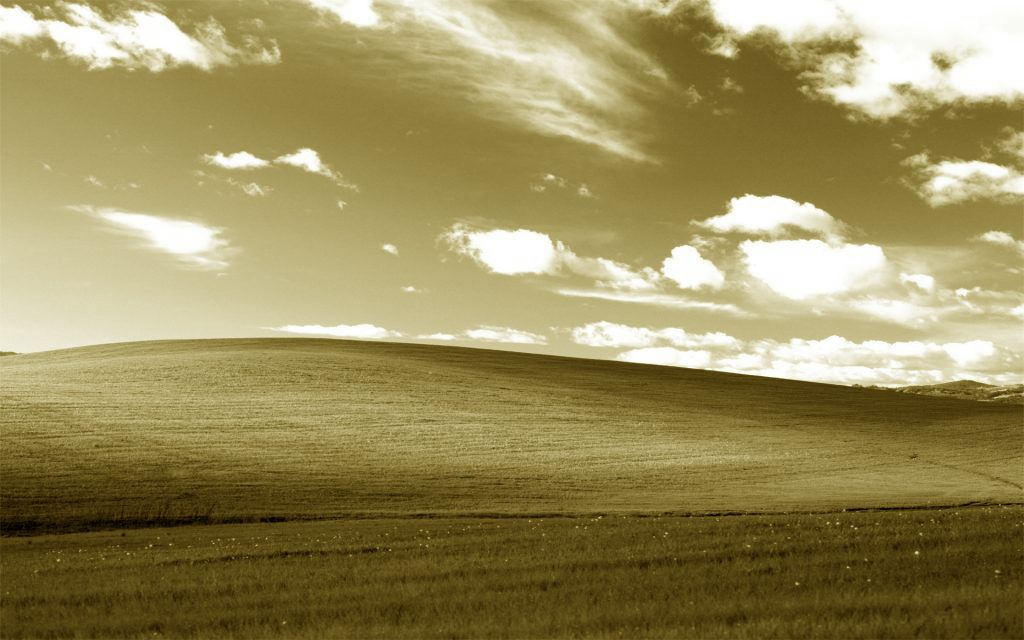
\includegraphics[angle=10, width=5cm]{kep2.jpg}
    \caption{2. kép}
    \label{fig:subfig2}
  \end{subfigure}
  \caption{2 Kép.}
  \label{fig:mainfig}
\end{figure}
\begin{tabular}{l||r|c|l|}
{} & egy & kettő & három\\
\hline
\hline
Hello & négy & öt & hat\\
világ! & {} & {} & {}\\
\cline{2-4}
{} & hét & nyolc & kilenc\\
\cline{2-2} \cline{4-4}
lorum & tíz & {} & tizenegy\\
ippse & {} & {} & {}\\
\hline
\end{tabular}
\\
\\
\\
\begin{tabular}{r|c|l}
1 & 2 & 3\\
\hline
\rowcolor{yellow}
4 & 5 & 6\\
\rowcolor{green}
7 & 8 & 9\\
\rowcolor{blue}
10 & {} & 11\\
\end{tabular}
\\
\\
\\
\begin{tabular}{r|cl}
\cellcolor{black}r{red}{egy} & kettő & három\\
\arrayrulecolor{green}
\hline	
\cellcolor{black}\textcolor{white}{a} & b & c\\
\cellcolor{black}\textcolor{white}{1} & 2 & \cellcolor{blue}3\\
\cellcolor{brown}\textcolor{white}{x} & {} & y\\
\end{tabular}
\end{document}